\chapter{区块链网络节点云化方案}

本章首先通过快速评审获得Kubernetes Operator赋能质量属性的策略集,  随后阐述区块链云化框架的设计原则, 最后结合区块链去中心化等特性以及设计原则分析筛选策略集形成面向Hyperledger Fabric的区块链网络节点云化的核心具体实施方案。

\section{快速评审}\label{section: rapid_reviews}

软件工程中, 快速评审(Rapid Review)是一种轻量级的二级研究, 以实践为导向专注于及时向研究人员提供证据\cite{cartaxo2020rapid}。本文对已发表的学术文章进行快速评审, 快速评审的目的是为了在较短时间内了解目前学术界使用Kubernetes Operator进行云化的现状, 以及如何使用Kubernetes对现有系统进行赋能。随后, 本文对快速评审所得到的结果进行整理归纳得到Kubernetes Operator如何为质量属性赋能的策略集。

本文的快速评审过程分为以下步骤: 首先进行自动化的全文数据库检索, 再筛选出与Kubernetes Operator及架构改造强相关的文献, 接下来提取出质量属性及相关策略, 最后归纳整理出策略集。

{\footnotesize
\begin{longtable}[h]{m{60pt} m{210pt} m{40pt}<{\centering}}
    \caption[每个全文数据库的搜索字符串]{每个全文数据库的搜索字符串} \label{search_string} \\
        \toprule  
        \textbf{全文数据库}&\textbf{搜索字符串}&\textbf{文献数}\\
        \hline
        IEEE Xplore &(“kubernetes AND operator”) OR (“k8s AND operator”) OR (“custom resource definition”) & 23 \\

        ACM & “kubernetes operator” OR “k8s operator” & 7 \\

        Springer &((“kubernetes AND operator”) OR (“k8s AND operator”))AND ((“custom resource definition”) OR "CRD") & 0 \\

        ScienceDirect &(“kubernetes AND operator”) OR (“k8s AND operator”) OR (“custom resource definition”) & 0 \\
        \hline
        Scopus\&Google &“kubernetes operator”& 21(去重) \\
        \bottomrule
    \end{longtable}
}

如表\ref{search_string}所示, 为全面获取学术届对基于Kubernetes Operator云化的策略, 确定了本次检索的全文数据库以及搜索字符串。本次检索主要针对计算机与软件工程领域的全文数据库\cite{lisboa2010systematic}(包含ACM、IEEE Xplore、Springer、ScienceDirect), 同时检索Scopus以及谷歌学术进行补充。最终, 本文围绕“kubernetes operator”为检索主题共得到51篇论文。在文献筛选阶段, 本文根据筛选标准筛选出15篇与Kubernetes Operator云化强相关的文献, 入选文献如表\ref{rapid_reviews}所示。文献筛选标准主要有:

\begin{itemize}[itemindent=2em]
    \item 论文的主要目的是利用Kubernetes对原有系统进行云化;

    \item 论文针对于Kubernetes Operator方法;

    \item 论文介绍了具体的改造策略及相关的质量属性。
\end{itemize}

{\footnotesize
\begin{longtable}[h]{m{40pt} m{280pt} m{40pt}<{\centering}}
    \caption[快速评审入选文献列表]{快速评审入选文献列表} \label{rapid_reviews} \\
        \toprule  
        \textbf{文献编号}&\textbf{文献标题}&\textbf{文献引用}\\
        \hline
        [P1]&Enhancement of observability using Kubernetes operator&\cite{Shenoy2022496}\\
        
        [P2]&Designing a Kubernetes Operator for Machine Learning Applications&\cite{kanso2021designing}\\
        
        [P3]&Container orchestration on HPC systems through Kubernetes&\cite{zhou2021container}\\
        
        [P4]&Validation and Benchmarking of CNFs in OSM for pure Cloud Native applications in 5G and beyond&\cite{pino2021validation}\\
        
        [P5]&On-the-fly fusion of remotely-sensed big data using an elastic computing paradigm with a containerized spark engine on kubernetes&\cite{huang2021fly}\\
        
        [P6]&A Role-Based Orchestration Approach for Cloud Applications&\cite{yue2021role}\\
        
        [P7]&A Design of MANO System for Cloud Native Infrastructure&\cite{lee2021design}\\
        
        [P8]&Dynamic Updates of Virtual PLCs Deployed as Kubernetes Microservices&\cite{koziolek2021dynamic}\\

        [P9]&Suture: Stitching safety onto kubernetes operators&\cite{mahajan2020suture}\\
        
        [P10]&Automation of virtualized 5G infrastructure using mosaic 5G operator over kubernetes supporting network slicing&\cite{wiranata2020automation}\\
        
        [P11]&5G Cloud-Native: Network Management \& Automation&\cite{arouk20205g}\\
        
        [P12]&Proposed model for distributed storage automation system using kubernetes operators&\cite{sharma2020proposed}\\
      
        [P13]&Monitoring Resilience in a Rook-managed Containerized Cloud Storage System&\cite{baumann2019monitoring}\\
        
        [P14]&Reproducible Benchmarking of Cloud-Native Applications With the Kubernetes Operator Pattern&\cite{henning2021reproducible}\\
        
        [P15]&Pivotal Greenplum©for Kubernetes: Demonstration of Managing Greenplum Database on Kubernetes&\cite{patel2019pivotal}\\
        \bottomrule
    \end{longtable}
}

在数据提取阶段, 本文对5个提取项(文献标题、文献发表年份、质量属性、策略、所属领域)进行抽取, 共得到44条针对不同质量属性的相关策略。在数据归纳阶段, 由于不同的文献中对语义相同的质量属性用词存在明显差异, 本文根据国际软件质量评价标准ISO/IEC 25010:2011\footnotemark[1]\footnotetext[1]{\href{https://www.iso.org/standard/35733.html}{ISO/IEC 25010:2011 System and software quality models}}所定义的质量模型对收集到的文献中表述的质量属性进行映射, 同时对相同或相似的策略进行整理合并, 得到策略集如表\ref{policy_set}所示。

{\footnotesize
\begin{longtable}[h]{m{40pt}|m{40pt}|m{20pt}|m{130pt}|m{100pt}}
    \caption[Kubernetes Operator云化策略集]{Kubernetes Operator云化策略集} \label{policy_set} \\  
        \hline
        \textbf{文献中质量属性}&\textbf{ISO质量属性}&\textbf{编号}&\textbf{策略}&\textbf{参考文献}\\
        \hline
        可迁移性 & 可移植性
        &T1&沙盒 & [P1-P3, P7-P8, P10-P12] \\\cline{3-5}

        \hline
        \multirow{3}*{可用性} & \multirow{3}*{可靠性}
        &T2&升级重启 & [P2, P15] \\\cline{3-5}
        & &T3&主备切换 & [P15] \\\cline{3-5}
        & &T4&监控 & [P1, P5, P12, P13] \\\cline{3-5}

        \hline
        \multirow{2}*{\parbox[c]{40pt}{生产效率}} & \multirow{2}*{易用性}
        &T5&支持用户初始化 & [P1, P2, P12-P15] \\\cline{3-5}
        & &T6&支持系统初始化 & [P1, P4, P13] \\\cline{3-5}

        \hline
        \multirow{2}*{\parbox[c]{40pt}{可扩展性}} & \multirow{2}*{无}
        &T7&基于监控指标的伸缩处理 & [P2, P6, P13] \\\cline{3-5}
        & &T8&数据分发 & [P15] \\\cline{3-5}

        \hline
        \multirow{3}*{安全性} & \multirow{3}*{安全性}
        &T9&限制访问 & [P2, P9] \\\cline{3-5}
        & &T10&认证授权 & [P3, P13] \\\cline{3-5}
        & &T11&分离实体 & [P9, P13] \\\cline{3-5}
        \hline
    \end{longtable} 
}



\section{设计原则}\label{section: framework_characteristics}

区块链云化框架致力于在BaaS一站式构建、管理、托管和运维区块链网络及其应用的基础上更深入云原生底层基础设施Kubernetes的底层, 有效利用云能力对HF基础设施节点赋能。BaaS在设计上以简单易用、成熟可扩展、安全可靠、可视运维等为主要方向\footnotemark[2]\footnotetext[2]{\href{http://www.caict.ac.cn/kxyj/qwfb/bps/201901/P020190111409291959654.pdf}{2019区块链即服务平台BaaS白皮书}}。区块链云化框架需要在上述设计原则的基础上进行适配与拓展:

\begin{itemize}[itemindent=2em]
    \item 简单易用: BaaS平台需要具备帮助企业实现自动配置, 快速启动区块链的能力。区块链云化框架需要在Kubernetes上完成HF的全生命周期管理。在Kubernetes上启动管理HF网络并部署链码需要专业的领域知识, HF各节点的配置项繁多且与Kubernetes适配极易出错。区块链云化框架需屏蔽底层HF配置与Kubernetes逻辑, 帮助用户采用命令行配置的方式提供完整的HF各组件的全生命周期管理;

    \item 灵活扩展: BaaS平台设计应采用抽象架构以及可插拔的模块。在此原则上, 区块链云化框架需按照模块化配置, 将Kubernetes底层的计算资源、存储资源、网络资源等供给HF, HF的Ca、Peer、Orderer基本节点的证书认证、共识、TLS加密、存储等功能模块作为可配置项进行命令式配置; 区块链云化框架需要能够确保系统核心底层逻辑稳定运行的同时, 对外提供小而精的扩展边界, 实现系统的高内聚与低耦合;

    \item 安全可靠: BaaS平台应具备有效的安全机制保证区块链服务的安全性。 区块链云化框架为满足上述原则, 需要具备有效的认证、鉴权、准入机制来确保区块链系统的安全性; 具备可插拔的共识算法确保区块链的去中心化、可追溯等特点, 支持完善的用户密钥授权、保存、隔离处理以及提供可靠的故障恢复能力;

    \item 可视运维: BaaS平台要提供必要的运维接口和运维授权的能力。当前区块链系统缺乏一套涵盖不同层面的标准方法来监控区块链及其智能合约的运行。 区块链云化框架需提供基本运维能力, 有效复用云上监控方案为区块链系统提供7*24小时可视化资源监控能力;

    \item 云链结合: BaaS平台需要结合云平台提供各种区块链所需的丰富资源。在此原则之上, 区块链云化框架需要具备高可迁移性, 具备基础架构的云独立性。本框架依托Kubernetes, 需要具备迁移到支持Kubernetes任何云的能力;

    \item 合作开放: BaaS平台应该和各个行业伙伴共同打造行业可信的区块链生态。为此, 区块链云化框架应该具备反馈机制的透明性。区块链云化框架需保证区块链上所有的交易记录是可追溯的、不可篡改的, 区块链交易过程以及获取交易产生的记录需要专业人员才能获取操作, 非专业人员难以理解, 框架需通过简单透明的方式获取交易记录。
\end{itemize}

\section{策略集应用}\label{section: policy_set_application}

通过快速评审的方式形成的基于Kubernetes Operator云化策略集作为指导方案, 需要贴合区块链领域自身约束才能有效纳入区块链云化框架中落地。本节将围绕“所选策略为何能提升质量属性”以及“所选策略是否适用于HF”进行阐述。

\textbf{T1: 沙盒}

\textbf{原理: }沙盒将系统实例与现实世界隔离开来, 使系统运作能够消除现实世界的影响, 虚拟机与容器化都提供了沙盒的能力。 相较于虚拟机而言, 容器化在云原生应用程序中的拥有更高的部署效率\cite{zhou2021container}、可迁移性。容器化可以使每个软件应用程序在隔离的环境中运行, 其将应用程序及库、配置文件和其他依赖项封装在一起, 确保了环境兼容性, 从而使用户能够轻松地在不同的环境中移动和部署程序。因此, 容器化使得应用程序具备极强的可移植性。Docker\footnotemark[1]\footnotetext[1]{\href{https://www.docker.com/}{Docker官网}}是容器化的典型代表, 其可以将运行态的容器打包成镜像(image)并储存在在线存储仓库中。Docker容器不是虚拟机, 这意味着它可以使用宿主机现有的网络接口\cite{shah2019building}。一旦创建了容器, 就可以为容器提供一个专用回环接口, 用于内部通信, 完成部署。

\textbf{适配性: }HF官方提供了Binaries和Docker镜像两种安装方式\footnotemark[2]\footnotetext[2]{\href{https://github.com/hyperledger/fabric/blob/main/scripts/bootstrap.sh}{fabric\_bootstrap.sh}}, 其天然满足容器化构建。

\textbf{T2: 升级重启}

\textbf{原理: }当系统某部分发生故障时, 需要能够快速的从故障中重新引入新的可用组件。Kubernetes作为容器管理调度平台, 其具备自恢复能力。Kubernetes会自动打包应用程序, 并根据预设需求运行Pod并管理容器。Pod内置标准的自重启策略的字段(restartPolicy), 首先Kubernetes会对Pod进行健康检查, 若存在故障则根据Pod的自重启策略对其进行重启。利用这种机制, 可以自动重启在执行过程中失败的容器, 并杀死那些没有响应用户定义的健康检查的容器。但如果节点本身死亡, 那么它会替换并重新安排发生故障的容器到其他可用节点上。

\textbf{适配性: }根据T1, HF网络采用容器化构建, 自然就可以通过Kubernetes托管。然而, 托管于Kubernetes需要从零开始为HF不同类型的网络节点提供编写多种的资源对象, 包含但不限于Deployment、Service等。一旦HF网络节点托管于Kubernetes, 即可原生地利用Kubernetes进行高可用的管理。


\textbf{T3: 主备切换}

\textbf{原理: } 在具备严格高可用的系统中, 往往需要处理主备切换。主节点就是提供服务的节点, 备份节点就是不提供服务的控制节点。所谓的主备切换就是当主节点故障时, 系统自动切换备份节点接管服务。要保证主备切换往往涉及到多种复杂的机制, 如数据同步、探活、网络切换等。所有冗余组件并行响应事件, 所有组件都处于相同状态。但响应只使用了一个组件, 其余组件被丢弃。当发生故障时, 停机时间通常不存在, 因为备份是当前的, 唯一的时间是恢复时间。Kubernetes Operator可以协助实现目标系统的主备切换任务, 并不丢失数据。

\textbf{适配性: }区块链网络是去中心化的网络, 所有的节点共同参与记账, 只需要网络中的大多数(超过51\%)节点的账本状态一致即可, 并不需要所有网络中的所有的Peer节点时刻保持高可用状态。针对于Peer的主备切换意义并不大, 针对Orderer的主备切换目前仍然是研究的空白。

\textbf{T4: 监控}

\textbf{原理: }Prometheus\cite{sukhija2019towards}作为云原生领域的监控事实标准, 其是一个时序数据库又是一个监控系统, 有着强大的功能和良好的生态。Grafana可以与各种其他类似于Prometheus的数据源进行交互并进行可视化。基于Prometheus的监控体系可以收集开放的监控指标并进行多维度数据模型的灵活查询, 极大增强了被监测系统的可监控性。

\textbf{适配性: } Mahajan等人\cite{mahajan2020suture}指出, 只有58\%的人认为他们有工具来理解Operator在异常情况下的行为, 并且他们强调了对Operator事件日志与监控的不满。HF网络各节点的运行终态是Pod, 利用Prometheus监控体系可以无侵入式的收集HF网络各节点的监控指标, 并将指标数据以Grafana图表的方式展示, 做到7*24小时可视运维。


\textbf{T5: 支持用户初始化}

\textbf{原理: }支持用户初始化, 即支持用户纠正错误或提高效率。框架需要帮助用户自动化配置HF领域知识, 提升用户启动HF网络的效率。Kubernetes Operator提供的CRD方式可以插拔式地将领域知识注入进云基础设施内部, CRD就是领域专家自定义的资源范式, 其规定了领域资源应该具备何种属性。特定领域专家编写的CRD能够注册进入集群, 注册之后领域的开发人员即可以根据CRD定义的属性编写特定于自身业务的CR。CRD降低了集群管理人员对HF网络的二次学习成本, 集群管理人员无需了解特定领域的领域知识, 仅需要通过kubectl原生的方式即可管理陌生领域的应用程序。

\textbf{适配性: }可以将HF网络节点通过CRD注册进入Kubernetes, 然而这存在一定的复杂性。编写HF领域CRD需要根据各网络节点的配置\footnotemark[1]\footnotetext[1]{\href{https://github.com/hyperledger/fabric-ca/blob/main/cmd/fabric-ca-server/config.go}{Ca Config}}\footnotemark[2]\footnotetext[2]{\href{https://github.com/hyperledger/fabric/blob/main/sampleconfig/orderer.yaml}{Orderer Config}}\footnotemark[3]\footnotetext[3]{\href{https://github.com/hyperledger/fabric/blob/main/sampleconfig/core.yaml}{Peer Config}}以及网络预期状态设计注入的属性。以Ca为例, 其存在22种一级配置项, 在编写Ca CRD时就需要对这些配置项进行甄别与筛选, 选取出适合插拔配置以及使用频率较高的配置并利用编程语言对其进行编写转换。

\textbf{T6: 支持系统初始化}

\textbf{原理: }本策略需要做到支持用于预测自身行为或用户意图的模型, 具体表现为: 框架可以维护一个任务模型, 这能够使得框架了解用户正在尝试什么并实时提供反馈。本框架可以利用Operator与Helm相结合的方式, 通过Controller协调机制时刻监听用户CR的状态并将状态更新到Helm最终反馈到集群中。
由于Helm能够自动化地在Kubernetes内构建部署应用程序, 但这是一个一次性部署动作, 仅仅完成了一次性自动化构建、部署HF网络的任务。本质上与现有Blockchain Automation Framework采用脚本方式部署无异, 这虽然能在一定程度上提升HF网络的部署效率, 但这无法将HF复杂的领域知识以插拔化的方式配置进入云基础设施内部。通过Operator与HF Helm的结合, 不仅能够提升HF网络的部署效率, 也可以时刻监听Helm状态实现对整个网络进行完整生命周期管理。

\textbf{适配性: } 根据T2, 将HF网络托管于Kubernetes就需要为其配置资源对象。一种是分别配置所需资源对象, 其次就是利用Helm为HF网络节点配置资源对象模板。若采用Helm, 需要利用模版语言配置HF网络节点, 并在Operator中对模板进行填充。


\textbf{T7: 基于监控指标的伸缩处理}

\textbf{原理: } 自动弹性伸缩能够基于资源使用情况对工作负载进行伸缩处理。 Kubernetes具备强大的伸缩能力, 其可以自动打包应用程序, 并根据预设需求运行Pod并管理容器。利用自身机制, Kubernetes可以轻松根据CPU、内存对工作负载进行横向扩容(Horizontal Pod Autoscaler, 简称HPA)或纵向扩容(Vertical Pod Autoscaler, 简称VPA)。但是, 在多种场景中需要按照业务监控指标进行扩容所容操作, 本策略能够利用定时的方式, 在Operator中收集业务监控指标对目标工作负载进行多副本的伸缩处理。

\textbf{适配性: } 无论是基于Kubernetes的多副本伸缩还是基于监控指标进行伸缩仅保证的是无状态应用的高可用性, 并不解决数据一致性问题, 所以为某个Pod节点增加多副本进行可伸缩意义不大, 利用Kubernetes的自恢复能力保证单Pod节点可用即可。

\textbf{T8: 数据分发}

\textbf{原理: } 虽然针对Peer节点的可伸缩性意义不大, 但从海量数据存储的角度来看, 使用云存储是加强区块链网络存储一种替代方法, 它减少了因区块存储空间有限而造成的限制\cite{gai2020blockchain}。云可以为区块链网络提供存储即服务(Storage as a Service, 简称SaaS)作为一种可扩展的链外解决方案。Kubernetes的SaaS通过服务的形式精细化使用存储资源, 实现了对存储定义(PVC)和存储申请(StorageClass)的灵活分离。这种链外存储机制可以使得HF网络能够通过Kubernetes的SaaS机制挂载外部存储单元而不必关心存储资源的实际物理位置, 能够做到存储资源的即插即用。 

\textbf{适配性: }HF网络的世界状态是一种脱链的链外附加缓存机制, 其最终被保存在链外的LevelDB或CouchDB中。同时, 世界状态的丢失并不会对区块链中的数据产生影响。除世界状态的存储, 针对网络节点以及链码的存储都可以通过定制“PVC+StorageClass”机制对外进行挂载。

\textbf{T9: 限制访问}

\textbf{原理: }访问控制是提供云数据安全和隐私的一种基本方法, 可以防止未经授权的用户侵入云数据。不可靠的访问控制方法也会影响其他功能, 如身份验证、授权和数据审核。除自定义访问控制机制外, 云中的传统访问控制方法主要基于成熟的访问控制策略, 现有的传统访问控制策略分为四种: 自主访问控制(Discretionary Access Control, 简称DAC)、强制访问控制(Mandatory Access Control, 简称MAC)、基于角色的访问控制(Role-Based Access Control, 简称RBAC)和基于属性的访问控制(Attribute-Based Access Control, 简称ABAC), 其对比如表\ref{access_control}所示。

{\footnotesize
\begin{longtable}[h]{m{20pt} m{200pt} m{60pt} m{60pt}}
    \caption[访问控制机制]{访问控制机制} \label{access_control} \\
        \toprule  
        \textbf{名称}&\textbf{机制}&\textbf{优点}&\textbf{缺点}\\
        \hline
        DAC & 根据被操作对象的权限控制列表或者权限控制矩阵决定用户的是否能对其进行操作 & 操作简单 & 权限控制分散, 不利于管理 \\

        MAC & 每个对象含有权限标识, 每个用户也含有权限标识, 用户能够操作对象取决于双方权限标识的关系 & 适合机密或等级严格的场景 & 缺乏灵活性 \\

        RBAC & 一个用户关联一个或多个角色, 一个角色关联一个或多个权限, 根据权限需要创建角色并与用户绑定 & 灵活易扩展、职责分离 & 未提供操作顺序控制机制 \\

        ABAC & 根据规则动态计算一个或一组属性是否满足某种规则并授权判断 & 集中管理、按需实现不同粒度权限控制 & 不直观、规则复杂过多会出现性能问题 \\
        \bottomrule
    \end{longtable}
}

云化框架需要在Kubernetes上部署HF节点和管理HF网络, 需要限制Kubernetes上其他用户对HF网络节点运行时的权限。在DAC中, 合法用户(如云服务提供商)根据自主访问控制策略来允许其他用户(如云用户)访问操作对象\cite{lopez2018access}, 同时阻止非授权的用户访问。DAC操作简单, 云用户能够进行灵活的访问控制, 然而DAC不需要严格的规则造成了权限管理的过于分散, 不利于综合管理; MAC则解决了DAC权限控制过于分散的问题, MAC是通过预定义的信任策略实现且该策略不能动态更改, 目标是限制访问的用户对目标对象的操作能力, MAC过于强调保密性, 管理缺乏灵活性; ABAC将访问规则写在配置文件里以实现多粒度的权限控制, 但是由于定义权限时不易看出用户和对象间的关系, 很容易给集群管理者带来运维上的麻烦; RBAC基于角色的权限控制体系, 能够实现“以岗定人”的目标。


\textbf{适配性: }Mahajan等人\cite{mahajan2020suture}指出, 47\%的Operator缺乏安全性的配置。利用RBAC可以从Kubernetes层面对HF网络节点添加安全权限机制。虽然RBAC没有提供顺序操作的控制机制, 但能兼容Kubernetes, 有效的为操作HF网络各类节点提供安全保证机制, 防止集群中其他用户恶意增删HF节点。若现有的访问控制机制不能满足需求, 可以创建自定义的访问控制机制实现更加符合业务实践的安全权限管理。

\textbf{T10: 认证授权}

\textbf{原理: }在设计软件系统时, 需要考虑如何让应用在各种复杂的环境中保证安全的访问。这中间涉及到针对用户的认证、授权。认证意味着系统识别合法用户, 如通过账号密码进行登录认证; 授权则是认证通过之后合法用户在系统中所能处理的问题。常见的认证包括信道SSL/TLS上的认证、协议HTTP上的认证以及内容Web上的认证, 常见的授权机制包括T9提到的访问控制机制授权以及OAuth2授权等。

\textbf{适配性: }由于HF网络是基于MSP的认证性网络, 是基于SSL/TLS的认证机制, 这种机制可以保护HF网络内部交易流程的安全性。这个过程包含了加密算法、生成密钥、公钥的分发、Ca认证、签名验证等各项复杂的过程, 所有的HF网络的参与者都需要提供可认证的身份信息, 即HF网络利用SSL/TLS作为本身的多用户认证授权的机制。云化框架需要自动化的兼容基于TLS的认证机制, 除此之外, 传统手动生成的HF网络密钥以文件的形式保存, 增加了密钥泄漏的风险, 云化框架需要结合HF的SSL/TLS机制提供安全的证书管理策略。


\textbf{T11: 分离实体}

\textbf{原理: }使用Namespace来隔离实体工作负载是一项基本的安全最佳实践。若不通过Namespace进行项目级别的资源隔离, Kubernetes中所有的工作负载是可以相互访问的。Kubernetes可以将内部的资源划分到不同的Namespace中以形成逻辑上的隔离。同一Namespace下的进程可以感受彼此的存在, 而对外界一无所知, 这可以实现与其他工作负载的资源与安全性隔离。

\textbf{适配性: }尽管Namespace是官方的简易强制执行资源隔离的方式。Mahajan等人\cite{mahajan2020suture}指出, 48\%的受访者报告称在生产中使用了多个Operator, 但只有三分之一的受访者表示他们使用了标准的资源隔离技术。可以通过结合T9的RBAC将HF网络放在单独的Namespace下交给不同的角色进行管理, 这有利于增强HF网络的资源安全性以及访问控制安全性。

除上述策略外, HF致力于构建透明、公开、去中心化的企业级分布式应用, 区块链云化框架需要在以下方面满足透明性原则。首先, 区块链云化框架构建HF网络过程的透明性, 区块链云化框架需要具备完备的日志体系, 日志能够提供记录区块链云化框架操作HF网络的行为以及网络状态, 并能够规范的表达出来; 其次, 对于链上交易而言, HF网络本就是公开透明的。 区块链云化框架不能屏蔽这一特性, 需要对HF网络账本具备更加简易、公开、透明的命令式查询渠道, 如命令式查询交易记录。

综上, 如图\ref{policy_set_application}所示, 在区块链HF网络场景下结合云化框架设计原则, 剔除了Kubernetes Operator云化策略集中不适用于HF网络的策略, 最终形成了面向Hyperledger Fabric的区块链网络节点云化框架的核心策略实施方案。

\begin{figure}[h] %figure环境,h默认参数是可以浮动,不是固定在当前位置。如果要不浮动,你就可以使用大写float宏包的H参数,固定图片在当前位置,禁止浮动。
    \centering %使图片居中显示
    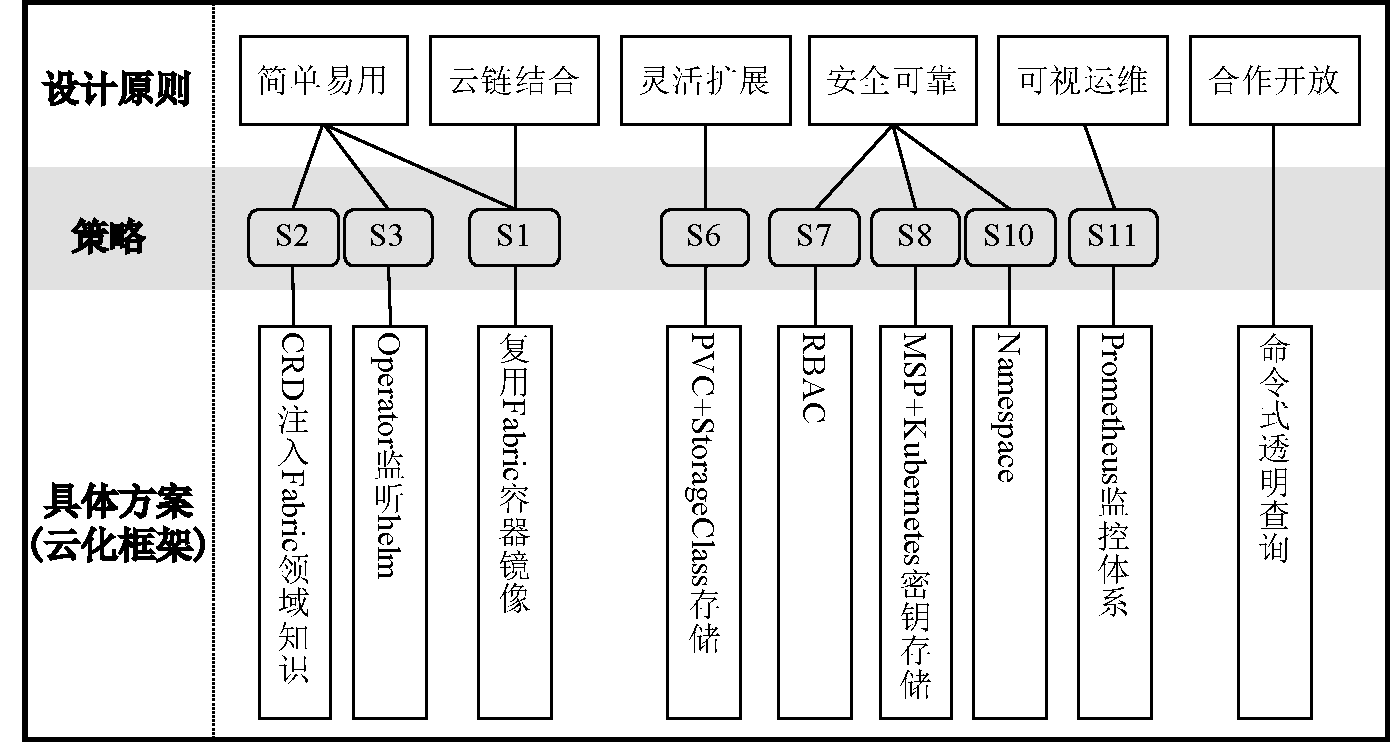
\includegraphics[width=1.0\textwidth]{FIGs/chapter3/policy_characteristics.pdf} %中括号中的参数是设置图片充满文档的大小,你也可以使用小数来缩小图片的尺寸。
    \caption{策略集应用} %caption是用来给图片加上图题的
    \label{policy_set_application} %这是添加标签,方便在文章中引用图片。
\end{figure}%figure环境


\section{本章小结}

首先详细介绍了快速评审的过程并得到基于Kubernetes Operator云化策略集;其次, 本章重点介绍了面向Hyperledger Fabric的区块链云化框架所应满足的设计原则; 最后结合HF网络特性以及区块链云化设计原则对策略集进行筛选, 形成了面向Hyperledger Fabric的区块链网络节点云化的核心策略实施方案。